%% Submissions for peer-review must enable line-numbering
%% using the lineno option in the \documentclass command.
%%
%% Preprints and camera-ready submissions do not need
%% line numbers, and should have this option removed.
%%
%% Please note that the line numbering option requires
%% version 1.1 or newer of the wlpeerj.cls file, and
%% the corresponding author info requires v1.2

\documentclass[fleqn,10pt,lineno]{wlpeerj} % for journal submissions

% ZNK -- Adding headers for pandoc

\setlength{\emergencystretch}{3em}
\providecommand{\tightlist}{
\setlength{\itemsep}{0pt}\setlength{\parskip}{0pt}}
\usepackage{lipsum}
\usepackage[unicode=true]{hyperref}
\usepackage{longtable}



\usepackage{lipsum}

\title{Recovery of mountain plant communities in response to reductions in
Nitrogen emissions is hidden by other drivers of global change}

\author[1, 2]{Tobias Roth}

\corrauthor[1, 2]{Tobias Roth}{\href{mailto:t.roth@unibas.ch}{\nolinkurl{t.roth@unibas.ch}}}
\author[2]{Lukas Kohli}

\author[3]{Beat Rihm}

\author[4]{Reto Meier}


\affil[1]{Zoological Institute, University of Basel, Basel, Switzerland}
\affil[2]{Hintermann Weber AG, Austrasse 2a, 4153 Reinach, Switzerland}
\affil[3]{Meteotest,Fabrikstrasse 14, 3012 Bern, Switzerland}
\affil[4]{Federal Office for the Environment (FOEN), Air Pollution Control and
Chemicals Division, 3003 Bern, Switzerland}


%
% \author[1]{First Author}
% \author[2]{Second Author}
% \affil[1]{Address of first author}
% \affil[2]{Address of second author}
% \corrauthor[1]{First Author}{f.author@email.com}

% 

\begin{abstract}
Nitrogen (N) deposition is a major threat to biodiversity of many
habitats. The recent introduction of cleaner technologies in Switzerland
has let to reductions in the emissions of nitrogen oxides, with
affiliated decrease in Nitrogen deposition. We infered different drivers
of community change (i.e.~Nitrogen deposition, climate warming, land-use
change) in Swiss mountain hay meadows. The data were obtained from the
Swiss biodiversity monitoring.
% Dummy abstract text. Dummy abstract text. Dummy abstract text. Dummy abstract text. Dummy abstract text. Dummy abstract text. Dummy abstract text. Dummy abstract text. Dummy abstract text. Dummy abstract text. Dummy abstract text.
\end{abstract}

\usepackage{amsthm}
\newtheorem{theorem}{Theorem}[section]
\newtheorem{lemma}{Lemma}[section]
\theoremstyle{definition}
\newtheorem{definition}{Definition}[section]
\newtheorem{corollary}{Corollary}[section]
\newtheorem{proposition}{Proposition}[section]
\theoremstyle{definition}
\newtheorem{example}{Example}[section]
\theoremstyle{definition}
\newtheorem{exercise}{Exercise}[section]
\theoremstyle{remark}
\newtheorem*{remark}{Remark}
\newtheorem*{solution}{Solution}
\begin{document}

\flushbottom
\maketitle
\thispagestyle{empty}

\section*{Introduction}\label{introduction}
\addcontentsline{toc}{section}{Introduction}

Nitrogen deposition is one of the major threats to biodiversity (Sala
2000, Bobbink 2010, Menier et al. 2016). Especially, there is strong
evidence for the reduction in diversity of species-rich grasslands in
Europe (Stevens et al. 2006, Maskell et al. 2010, Duprè et al. 2010).

Fertilizing experiments show that plant biodiversity in mountain
grasslands is negatively affected by nitrogen addition, too (Humbert et
al. 2016).

Since the late 1980s measures to reduce atmospheric pollution have
successfully reduced emissions of nitrogen oxides, with affiliated
decrease in Nitrogen deposition in many parts of Europe (Tørseth et al.,
2012, Maas and Grennfelt, 2016) {[}Tørseth et al.,: Atmos. Chem. Phys.,
12, 5447--5481, 2012{]}. However, it is an open question whether and how
fast the reduction in N deposition rates will lead to the recovery of
extant plant communities.

Quantifying the potential recovery of biodiversity in response to
reducing air pollution requires an alternative to the space-for-time
approach, ideally monitoring long-term community dynamics on permanent
plots (Duprã, C. et al. Changes in species richness and composition in
European acidic grasslands over the past 70 years: the contribution of
cumulative atmospheric nitrogen deposition. Glob. Change Biol. 16,
344--357, (2010).

One useful approach to understanding biodiversity change is through
estimates of biodiversity turnover reflecting both immigration and
extinction, often in a closed range of values (Hillebrand et
al-2018.pdf).

Observation data of vascular plants from field recordings shows negative
correlations of Nitrogen deposition with species richness and species
composition in mountain hay meadows (Roth et al. 2013).

In Switzerland, grassland accounts for 70 per cent of the agricultural
land. With extensive cultivation, permanent grassland has a very high
biodiversity. This applies in particular to the meadows of the Swiss
mountain region (Schlup et al. 2013). In the alpine region, meadows with
a high plant diversity are of great importance agronomically (Leiber et
al. 2005), for the image of the products and for the conservation of
biodiversity (Hohl, 2006).

The meta-analysis of Humbert et al. (2016) showed management and abiotic
factors to interact with nitrogen addition to drive plant community
changes: The overall effects of N addition on plant species richness and
diversity (Shannon index) were more pronounced in managed experimental
sites with warmer summers. Management regimes of accessible mountainous
areas are intensified, while poorly accessible mountainous areas are
being abandoned (Tasser and Tappeiner, 2002; Graf et al., 2014, Strebel
and Bühler, 2015). This change in traditional management regimes is
considered as a major driver that endangers grassland biodiversity in
mountainous regions of Europe (Niedrist et al., 2009; Homburger and
Hofer, 2012).

On European mountain summits, plants shifted upwards in the last decades
(Rumpf et al. 2018). The authors conclude that «These results suggest
that recent climate warming interacted with airborne nitrogen deposition
in driving the observed dynamics. As changes increased more for species
from lower elevations and eutrophic plant species showed the strongest
increase in abundance, these findings might be relevant for mountain hay
meadows, too.

\section*{Materials \& Methods}\label{materials-methods}
\addcontentsline{toc}{section}{Materials \& Methods}

\subsection*{Monitoring data and community
measures}\label{monitoring-data-and-community-measures}
\addcontentsline{toc}{subsection}{Monitoring data and community
measures}

We analysed the presence/absence of vascular plants sampled within the
scope of Switzerland's Biodiversity Monitoring (BDM) programme that was
launched in 2001 to monitor Switzerland's biodiversity and to comply
with the Convention on Biological Diversity of Rio de Janeiro (Weber,
Hintermann, and Zangger 2004). The sampling sites were circles with a
size of 10 m\(^2\) and data collection was carried out by qualified
botanists who visited each sampling site twice within the same season.
During each visit all the vascular plant species detected on the plot
were recorded. After the sampling of the plant data the botanists also
assigned a habitat type to each sampling site according to the
classification system developed for Switzerland (Delarze and Gonseth
2008).

We matched the habitat types of the Swiss classification system with the
categories from the EUNIS system (level-3 classification; Davies, Moss,
and Hill 2004) and selected all sampling sites in mountain hay meadows
(EUNIS E2.3) For more details on the field methods see Plattner, Birrer,
and Weber (2004), Roth et al. (2013) and Roth et al. (2017). We analysed
the data from 2003 to 2017. During that study period each sampling site
was surveyed once per five-year period: the first period lasted from
2003 to 2007, the second from 2008 to 2012 and the third from 2013 to
2017. These selection criteria resulted in sample of 129 sites.

For each survey (a survey consists of the two visits per season) we
calculated the following community measures: (1) The number of recorded
species (species richness), the community mean of indicator values of
recorded species for temperature (2), humidity (3), nutrients (4) and
light (5). The indicator values were obtained from the recalibrated
indicator values for the Swiss Flora (Landolt et al. 2010). Additionally
to these five community measures that describe the state of plant
communities for each site at a given time point, we also estimated the
temporal turnover (i.e.~species exchange ratio sensu Hillebrand et al.
(2018)) as the proportion of species that differ between two time points
to describe the community change between two time points.

\subsection*{Environmental gradients}\label{environmental-gradients}
\addcontentsline{toc}{subsection}{Environmental gradients}

We expected different global change patterns to simultaneously cause
temporal change in mountain hay communities. To better disentangle the
importance of these mechanisms we ordered the sites along four main
environmental gradients. First we expected communities to response to
climate warming and the response might be different depending along the
temperature gradient (Roth, Plattner, and Amrhein 2014). To describe the
temperature gradient we used the mean annual temperature per site from
the WordClim database (Fick and Hijmans 2017). Another key drivers for
plants that is likely to be affected by climate change is precipitation
(Beier et al. 2012). We used the annual precipitation per site from the
WordClim database (Fick and Hijmans 2017).Further, we estimated
atmospheric N deposition for each site using a pragmatic approach
described in Rihm and Kurz (2001) that combines monitoring data, spatial
interpolation methods, emission inventories, statistical dispersion
models and inferential deposition models. For details on the estimation
of N deposition see Rihm and Kurz (2001) and Roth et al. (2017). Finally
we used inclination as proxy for land-use intensity because we expected
that steeper sites are likely to be less intensively managed (Strebel
and Bühler 2015).

\subsection*{Statistical analyses}\label{statistical-analyses}
\addcontentsline{toc}{subsection}{Statistical analyses}

To estimate the linear trend over time for each of the five community
measures we applied linear mixed models (LMM) with normal distribution
except for species-richness with Poisson distribution and the logarithm
as link function. We specified site specific trends with the assumption
that the between-site differences in intercepts and slopes can be
described with normal distributions (i.e.~a random intercept random
slope model, {\textbf{???}}). Model parameters were estimated in a
Bayesian framework using the R-Package \emph{rstanarm} (Stan Development
Team 2016, Muth, Oravecz, and Gabry (2018)).

To infer whether species turnover was changing along the gradient, we
used a Binomial-LMM with the proportion of species that differed between
two surveys as dependent variable and the site gradients and period
(first/second vs.~second/third surveys) as predictors and site-ID as
random effect. Model parameters were estimated in a Bayesian framework
using the R-Package \emph{rstanarm} (Stan Development Team 2016, Muth,
Oravecz, and Gabry (2018)).

To infer whether species that colonized or disappeared from a site had
particular indicator values that differed from the other species at that
site, we produced for each site a list with all species that were
recorded during the three surveys (total community). We then calculated
the community mean (CM) of the indicator value for all species that
colonized the site during the three surveys (i.e.~not recorded during
first survey and recorded during second or not recorded during second
and recorded during third). We then randomly selected the same number of
species from the total community and also calculated the community mean
of the value for these species (random-CM). We repeated the random
selection of species 1000 times. Then we calculated the differences of
the CM minus the average of the random-CMs to obtain a standardized
measure (standardized-CM) of how different the disappearing species were
from random expectation. A standardized-CM \textless{} 0 would suggest
that the indicator value of colonizing species were lower than the
average species that were occurring at this site. We applied this method
for both colonizing and disappearing species and for the indicator
values for temperature, humidity, nutrients and light (see Appendix A).
We then inferred whether the standardized-CM is changing along the
corresponding gradient using linear models. Model parameters were
estimated in a Bayesian framework using the R-Package \emph{rstanarm}
(Stan Development Team 2016, Muth, Oravecz, and Gabry (2018)).

We used logistic-LMM to infer whether the colonization probability or
local survival probability was changing along the Nitrogen deposition
gradient and whether this changing depended on the species indicator
value for nutrients. To analyse the colonization probability we selected
all species that were not observed during the first survey, and asked if
they were observed (then Occ = 1) or not observed (then Occ = 0) during
the second survey. The same was also done for all species that were not
observed during the second survey. The variable `occ' was then used as
dependent variable in the logistic-LMM. As predictor variables the model
contained the Nitrogen deposition of the site, the indicator value for
nutrients of the species and the interaction of these two variables.
Additionally species-ID and site-ID were included as random effects. The
same logistic\_LMM was also used to infer local survival probability. In
that case, however, we selected all species that were recorded during
the first or second survey and the variable `occ' then indicated whether
or not the species was also observed during the next survey. Model
parameters were estimated using an approximate Bayesian approach using
the R-Package \emph{arm} (Gelman and Su 2018).

To estimate the effect of Nitrogen deposition on total species richness
at a given time point, we described the plant species richness at the
sites using a generalized linear model with Poisson distribution and the
logarithm as link function. As predictors we used the four environmental
gradients as described above. Model parameters were estimated using an
approximate Bayesian approach using the R-Package \emph{arm} (Gelman and
Su 2018).

\section*{Results}\label{results}
\addcontentsline{toc}{section}{Results}

\subsection*{Temporal change in community
structures}\label{temporal-change-in-community-structures}
\addcontentsline{toc}{subsection}{Temporal change in community
structures}

\begin{table}

\caption{\label{tab:communitytrendstab}Average measures of community structure for the three sampling periods (period 1: 2003-2007; period 2: 2008-2012; period: 2013-2017). The temporal trends are given as change per 10 years and were estimated from linear mixed models with normal distribution (except for species richness with Poisson distribution and a log-link function). The measure of precision for the temporal trend is given as the 5\% and 95\% quantiles of the marginal posterior distribution of the linear trend. The column 'Prob. for trend' gives the probability that the linear trend is $> 0$.}
\centering
\begin{tabular}[t]{lrrrrrrr}
\toprule
Measures & Period 1 & Period 2 & Period 3 & Trend & 5\% & 95\% & Prob. for trend\\
\midrule
Species-richness & 45.72 & 46.02 & 45.74 & 0.00 & -0.03 & 0.03 & 0.53\\
Temperature value & 3.11 & 3.13 & 3.13 & 0.01 & 0.00 & 0.03 & 0.97\\
Huminity value & 2.99 & 2.98 & 2.99 & 0.01 & -0.01 & 0.02 & 0.80\\
Nutrients value & 3.20 & 3.20 & 3.20 & 0.00 & -0.02 & 0.01 & 0.33\\
Light value & 3.56 & 3.55 & 3.55 & -0.01 & -0.02 & 0.00 & 0.07\\
\bottomrule
\end{tabular}
\end{table}

The five measures of plant community structure suggested that plant
communities in mountain hay meadows were rather stable between 2003 and
2017 and did not show a clear increase or decrease over time (Table
\ref{tab:communitytrendstab}): for each of the three 5-year survey
periods the averages of species-richness and the average indicator
values for temperature, humidity, nutrients and light did not vary much
among the three sampling periods and the estimated trends were rather
small. Except for average indicator value for temperature, the 90\%
credible-interval of the temporal trend contained zero. The results from
the linear mixed models suggest that a linear temporal change was most
likely for the community mean of the indicator value for temperature
(probability of increase: 0.97), followed by the community mean of the
indicator value for light (probability of decrease: 0.93) and it was
least likely for the species richness (probability of increase: 0.53).
The chance that the community mean of the nutrient value decreased
between 2003 and 2017 was 0.67.

\subsection*{Species turnover}\label{species-turnover}
\addcontentsline{toc}{subsection}{Species turnover}

\begin{table}

\caption{\label{tab:turnovertab}Change of species turnover along the four gradients. The slopes along the gradients (estimate) are given as the change per 10 years of the logit-probability of species that differed between two surveys. Estimates and the 5\% and 95\% quantiles of the marginal posterior distribution obtained from a Binomial-GLMM.}
\centering
\begin{tabular}[t]{lrrr}
\toprule
Gradient & Estimate & 5\% & 95\%\\
\midrule
Annual mean temperature & 0.04 & -0.02 & 0.10\\
Annual mean precipitation & -0.03 & -0.12 & 0.07\\
Nitrogen deposition & -0.14 & -0.30 & 0.02\\
Inclination & -0.03 & -0.10 & 0.03\\
\bottomrule
\end{tabular}
\end{table}

This temporal stability as inferred from the community measures was,
however, in contrast to a rather large observed temporal turnover of
species. The average percentage \(\pm\) SD of species that differed
between the first and second survey at a site was 37.65 \(\pm\) 10.43\%
and the percentage of species that differ between the second and third
survey was 35.66 \(\pm\) 10.36\%. Thus, it seemed that the turnover from
the first/second survey to the turnover of the second/third survey
moderately decreased (90\% Credible interval of the change in turnover
estimated from the Binomial generalized linear mixed model: -0.14 -
-0.03). Variation in species turnover was largest along the Nitrogen
deposition gradient with highest species turnover at sites with low
Nitrogen deposition (Table \ref{tab:turnovertab}). The other three
gradients were less important to explain the variation in species
turnover among sites.

\begin{table}

\caption{\label{tab:difffromrandomtab}Difference in the average indicator value of species that (a) disappeared from site or (b) newly colonized a site compared to the same number of species that were randomly selected from all species recorded at a site. Shown are the results from linear model with the difference between disappeard/colonized species and random species as dependend variable and the sitemeasure (gradient) as predictor variable.}
\centering
\begin{tabular}[t]{llcccccc}
\toprule
\multicolumn{2}{c}{ } & \multicolumn{3}{c}{Difference from random} & \multicolumn{3}{c}{Change along gradient} \\
\cmidrule(l{2pt}r{2pt}){3-5} \cmidrule(l{2pt}r{2pt}){6-8}
Ellenberg value & Gradient & Estimate & 5\% & 90\% & Estimate & 5\% & 90\%\\
\midrule
\addlinespace[0.3em]
\multicolumn{8}{l}{\textit{(a) Plants that disappeard from a site}}\\
\hspace{1em}Temperature & Annual mean temperature & -0.012 & -0.034 & 0.011 & 0.007 & -0.002 & 0.017\\
\hspace{1em}Humidity & Annual mean precipitation & -0.006 & -0.042 & 0.032 & 0.011 & -0.010 & 0.032\\
\hspace{1em}Nutrients & Nitrogen deposition & -0.024 & -0.059 & 0.011 & 0.013 & -0.028 & 0.054\\
\hspace{1em}Light & Inclination & -0.023 & -0.050 & 0.003 & -0.002 & -0.026 & 0.021\\
\addlinespace[0.3em]
\multicolumn{8}{l}{\textit{(b) Plants that newly colonized a site}}\\
\hspace{1em}Temperature & Annual mean temperature & 0.016 & 0.000 & 0.033 & -0.001 & -0.008 & 0.006\\
\hspace{1em}Humidity & Annual mean precipitation & 0.020 & -0.013 & 0.051 & -0.003 & -0.021 & 0.016\\
\hspace{1em}Nutrients & Nitrogen deposition & -0.076 & -0.108 & -0.042 & 0.060 & 0.022 & 0.098\\
\hspace{1em}Light & Inclination & -0.041 & -0.063 & -0.018 & 0.011 & -0.009 & 0.029\\
\bottomrule
\end{tabular}
\end{table}

High species turnover at a site is the result of species that
disappeared from the site and species that newly colonized the site. To
better understand the factors that drive these changes we are
particularly interested whether the species that disappeared or
colonized the sites differed in indicator values compared to what would
be expected if the same number of species randomly disappeared or
colonized the sites (i.e.~random disappearance and random colonization)
and whether there is a change along the gradients. It seems that the
indicator values of newly colonizing species differed more from random
colonization than the indicator values of disappearing species (Table
\ref{tab:difffromrandomtab}). For colonizing species, we found the
largest differences from random colonization in the indicator value for
nutrients: at sites with nitrogen deposition of 10 kg ha\(^{-1}\)
yr\(^{-1}\) the newly colonizing species had in average a lower
indicator value for nutrients than species under random disappearance
(column ``Difference from random'' in Table
\ref{tab:difffromrandomtab}), but this differences between colonizing
species and random colonization decreased with increasing Nitrogen
deposition (column ``Change along gradient'' in Table
\ref{tab:difffromrandomtab}). Thus at high Nitrogen deposition
colonizing species did not differ from random species (see Figure 3b in
Appendix A).

While colonizing species had higher temperature values compared to what
we would expect under random colonization, the differences between
colonizing species and random colonization was about four times smaller
compared to the difference in indicator value for nutrients between
colonizing species and random species. Nevertheless, the variation in
indicator value for temperature seemed important to explain the total
species turnover. This is because, disappearing species tend to have
lower temperature value than random species as well as colonizing
species tend to have higher temperature values than random species; both
processes lead to an overall replacement of species with lower
temperature value with species with higher temperature values. This was
not the case for the indicator value for nutrients: species with lower
nutrients values tended to be more likely to disappear from as well as
to colonize sites compared to random species (Table
\ref{tab:difffromrandomtab}). See also Appendix A were we present
detailed results for the comparison between colonizing or disappearing
species with randomly selected species.

\subsection*{Potential effects of reduction in Nitrogen
emmissions}\label{potential-effects-of-reduction-in-nitrogen-emmissions}
\addcontentsline{toc}{subsection}{Potential effects of reduction in
Nitrogen emmissions}

\begin{figure}
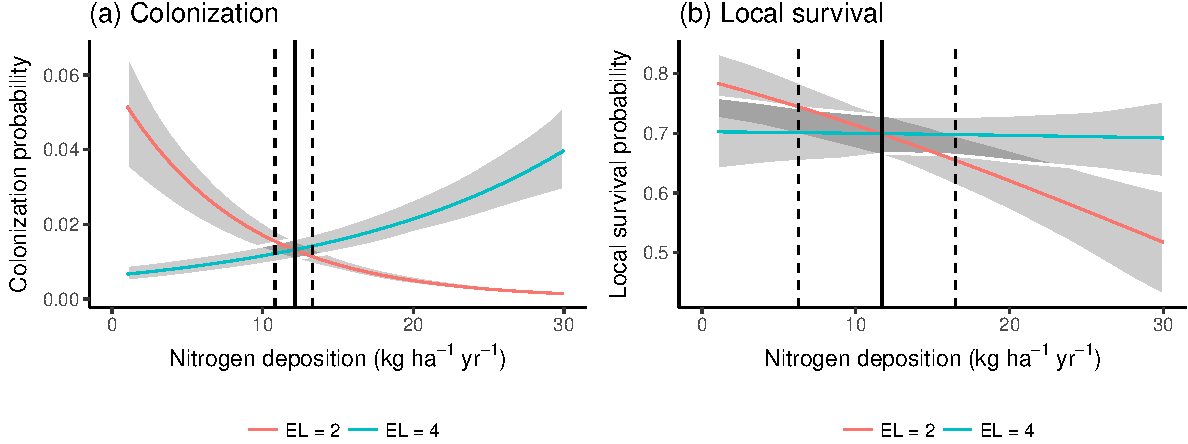
\includegraphics[width=1\linewidth]{Manuscript_files/figure-latex/cl-1} \caption{Colonization (a) and local survival (b) of oligotrophic (Ellenberg N = 2; red line) and eutrophic (Ellengerg N = 4) species along the N deposition gradient. Given are means and 95\%-Credible Intervals from logistic linear mixed models. The vertical lines indicat the deposition rate with equal colonization or survival probabilities for oligotrophic and eutrophic species with the solid line indicating the median and the dashed lines the 5\% and 95\% quantiels of the margional posterior distribution.}\label{fig:cl}
\end{figure}

In Fig. \ref{fig:cl} we compare the colonization and local survival
probability of oligotrophic (indicator value of nutrients = 2) and
eutrophic (indicator value of nutrients = 4) species along the Nitrogen
deposition gradient. Local survival probability was the same for
oligotrophic and euthrophic species at a deposition rate of 12.66 kg N
ha\(^{-1}\) yr\(^{-1}\); colonization probability was the same for for
oligotrophic and euthrophic species at a deposition rate of 12.22 kg N
ha\(^{-1}\) yr\(^{-1}\). In only 0.36\% of the sites the deposition rate
was below 12.5 kg N ha\(^{-1}\) yr\(^{-1}\) where the replacement of
eutrophic with oligotrophic species is likely.

While we could not detect a consistent decrease in average indicator
value for nutrients (Table \ref{tab:communitytrendstab}), the higher
colonization rate of species with low nutrient value at sites with low
deposition rate seems to affect the spatial variation of species
richness: sites with low Nitrogen deposition are likely to become more
species rich over time likely resulting in steeper slope of the negative
relationship between Nitrogen deposition and species richness. Indeed,
if we apply at different time points a similar model as in Roth et al.
(2013) to infer the effects of Nitrogen deposition on the spatial
variation of species richness, the resulting effect size (i.e.~the
slope) becomes more negative over time (Fig. \ref{fig:figconsequences}).

\begin{figure}
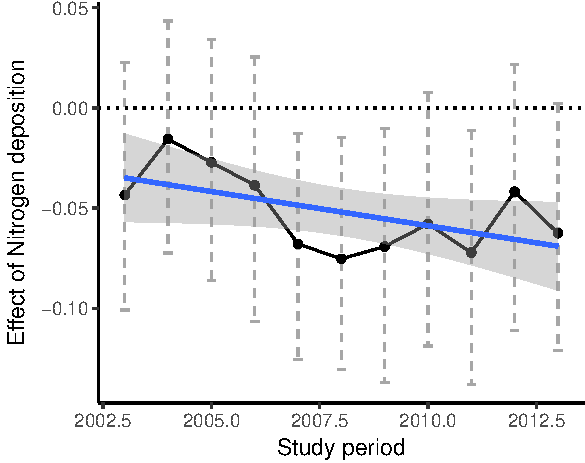
\includegraphics[width=0.5\linewidth]{Manuscript_files/figure-latex/figconsequences-1} \caption{Effect size of Nitrogen deposition on total species richness estimated from applying the Poisson-GLM with species richness as dependend variable and Nitrogen deposition plus other site covariates as predictors using only the surveys from one five-year interval. Note that within every five-year interval all plots were sampled once.}\label{fig:figconsequences}
\end{figure}

\section*{Discussion}\label{discussion}
\addcontentsline{toc}{section}{Discussion}

\begin{itemize}
\item
  \emph{General points}: Although N deposition considerably declined
  between 2005 and 2015, we could not detect major shifts in plant
  community structure during the same time period. Although NOx
  emissions in Switzerland decreased by 46\% between 1990 and 2010 and
  NH3 emissions by 14\% (Maas and Grennfelt, 2016), nitrogen deposition
  on our plots decreased by only 2.7 kg ha\(^{-1}\) yr\(^{-1}\) on
  average between 2000 and 2015 (Meteotest, 2018). This is only about
  one tenth of the decrease in England in the same period, where
  Nitrogen deposition decreased by 24kg ha\(^{-1}\) yr\(^{-1}\) from
  1996 to 2011 (Storkey et al. 2015). In 2015, average N deposition was
  14.8 kg ha\(^{-1}\) yr\(^{-1}\), about 85\% of 2000 deposition, and
  due to the rather short period of time and the small decrease in
  nitrogen deposition, it is not surprising that species richness has
  not reacted significantly.
\item
  \emph{Replacement of oligotrophic with eutrophic species is faster
  than the oposite direction}: Eutrophic species have rather high local
  survival across the entire deposition gradient, while oligotrophic
  species have much reduced local survival at high N deposition. This
  suggests that it takes more time to replace eutrophic by oligotrophic
  species than replacing oligotrophic by eutrophic species. Climatic
  effects may be more likely to be reversed than effects due to
  fertilization.
\item
  \emph{Methodological point}: The rather large spatial turnover might
  be partly explained by species that remained undetected in one of the
  surveys. From the randomly selected quality control of the BDM 17
  mountain hay meadows were investigated from 2003 to 2017. Species
  richness was surveyed in the same year by two independent botanists.
  The species match is (mean \(\pm\) SD) 85 \(\pm\) 5.2 per cent,
  suggesting that at least a portion of the turn over is due to agent
  effects. However, our results suggest that turnover is caused at least
  partly by species with specific indicator values. This deviation from
  what we would expect under random species turnover is unlikely to be
  explained by species that remained undetected.
\item
  \emph{Empirical critical loads}: Our data on colonization and local
  survival (i.e.~temporal variation) confirm the empirical critical
  loads that we inferred from analysing spatial co-variation of N
  deposition and species richness.
\item
  \emph{Space for time substitution}: Often observational studies infer
  the change of plant diversity along a gradient of N deposi- tion.
  Thus, they infer how the spatial variation in species richness is
  related to N deposition and assume that this spatial variation in
  species richness arose because over time some areas lost more species
  than others because they chronically experienced higher N deposition.
  Alt- hough there is evidence supporting the use of such a `space for
  time substitution' for detecting the effects of N deposition on plant
  diversity (Stevens et al. 2010), they can not replace stud- ies that
  relate temporal patterns in species with N deposition (De Schrijver et
  al. 2011). While recovery of acidified surface waters has been well
  investigated (De Vries et al. 2015), there are only a limited number
  of studies inferring temporal trends of plant species diversity relat-
  ed to varying amounts of N-deposition. Storkey et al. (2015)
  demonstrated a positive response of biodiversity to reducing N
  addition from either atmospheric pollution or fertilizers in the Park
  Grass Experiment: «The proportion of legumes, species richness and
  diversity increased across the experiment between 1991 and 2012 as
  N-deposition declined». For forest floor vegetation in permanent plots
  across Europe the exceedance of critical loads of N over a peri- od
  from 9 to 42 years had negative effects on the cover of oligotrophic
  plant species, i.e spe- cies that prefer nutrient-poor soils, although
  species richness remained constant (Dirnböck et al. 2014). Another
  example of recovery in eutrophicated habitats gives the recovery of
  species richness in previously fertilized plots (Clark and Tilman
  2008). In this study, the recorded recovery in species richness within
  one or two decade was likely due to the species rich vege- tation
  surrounding the experimental plots, from where immigration was easily
  feasible.
\end{itemize}

\section*{Conclusions}\label{conclusions}
\addcontentsline{toc}{section}{Conclusions}

xxx

\section*{Acknowledgements}\label{acknowledgements}
\addcontentsline{toc}{section}{Acknowledgements}

We thank the dedicated and qualified botanists who conducted fieldwork.
The Swiss Federal Office for the Environment (FOEN) kindly provided
biodiversity monitoring data and topographic data. This work was
supported by the FOEN, the Swiss National Science Foundation (grant no.
31003A\_156294), the Swiss Association Pro Petite Camargue Alsacienne,
the Fondation de bienfaisance Jeanne Lovioz, and the MAVA Foundation.

\section*{References}\label{references}
\addcontentsline{toc}{section}{References}

\hypertarget{refs}{}
\hypertarget{ref-Beier2012}{}
Beier, Claus, Carl Beierkuhnlein, Thomas Wohlgemuth, Josep Penuelas,
Bridget Emmett, Christian Körner, Hans Boeck, et al. 2012.
``Precipitation Manipulation Experiments--challenges and Recommendations
for the Future.'' \emph{Ecology Letters} 15 (8): 899--911.

\hypertarget{ref-Davies2004}{}
Davies, CE, D Moss, and MO Hill. 2004. ``EUNIS Habitat Classification,
Revised 2004. Report to European Environment Agency, European Topic
Centre on Nature Protection and Biodiversity.''

\hypertarget{ref-Delarze2008}{}
Delarze, Raymond, and Yves Gonseth. 2008. \emph{Lebensräume Der Schweiz:
Ökologie - Gefährdung - Kennarten}. Ott.
\url{https://books.google.ch/books?id=8kFrAAAACAAJ}.

\hypertarget{ref-Fick2017}{}
Fick, Stephen E, and Robert J Hijmans. 2017. ``WorldClim 2: New 1-Km
Spatial Resolution Climate Surfaces for Global Land Areas.''
\emph{International Journal of Climatology} 37 (12): 4302--15.

\hypertarget{ref-arm2018}{}
Gelman, Andrew, and Yu-Sung Su. 2018. \emph{Arm: Data Analysis Using
Regression and Multilevel/Hierarchical Models}.
\url{https://CRAN.R-project.org/package=arm}.

\hypertarget{ref-Hillebrand2018}{}
Hillebrand, Helmut, Bernd Blasius, Elizabeth T. Borer, Jonathan M.
Chase, John A. Downing, Britas Klemens Eriksson, Christopher T.
Filstrup, et al. 2018. ``Biodiversity Change Is Uncoupled from Species
Richness Trends: Consequences for Conservation and Monitoring.''
\emph{Journal of Applied Ecology} 55 (1): 169--84.
doi:\href{https://doi.org/10.1111/1365-2664.12959}{10.1111/1365-2664.12959}.

\hypertarget{ref-Landolt2010}{}
Landolt, Elias, Beat Bäumler, Andreas Erhardt, Otto Hegg, Frank Klötzli,
Walter Lämmler, Michael Nobis, et al. 2010. \emph{Flora Indicativa.
Ecological Inicator Values and Biological Attributes of the Flora of
Switzerland and the Alps.} Haupt Verlag.

\hypertarget{ref-Muth2018}{}
Muth, Chelsea, Zita Oravecz, and Jonah Gabry. 2018. ``User-Friendly
Bayesian Regression Modeling: A Tutorial with Rstanarm and Shinystan.''
\emph{The Quantitative Methods for Psychology} 14 (2): 99--119.

\hypertarget{ref-Plattner2004}{}
Plattner, Matthias, Stefan Birrer, and Darius Weber. 2004. ``Data
Quality in Monitoring Plant Species Richness in Switzerland.''
\emph{Community Ecology} 5 (1): 135--43.

\hypertarget{ref-Rihm2001}{}
Rihm, Beat, and Daniel Kurz. 2001. ``Deposition and Critical Loads of
Nitrogen in Switzerland.'' In \emph{Acid Rain 2000}, 1223--8.

\hypertarget{ref-Roth2013}{}
Roth, Tobias, Lukas Kohli, Beat Rihm, and Beat Achermann. 2013.
``Nitrogen Deposition Is Negatively Related to Species Richness and
Species Composition of Vascular Plants and Bryophytes in Swiss Mountain
Grassland.'' \emph{Agriculture, Ecosystems \& Environment} 178: 121--26.
doi:\href{https://doi.org/10.1016/j.agee.2013.07.002}{10.1016/j.agee.2013.07.002}.

\hypertarget{ref-Roth2017}{}
Roth, Tobias, Lukas Kohli, Beat Rihm, Reto Meier, and Beat Achermann.
2017. ``Using Change-Point Models to Estimate Empirical Critical Loads
for Nitrogen in Mountain Ecosystems.'' \emph{Environmental Pollution}
220: 1480--7.

\hypertarget{ref-Roth2014}{}
Roth, Tobias, Matthias Plattner, and Valentin Amrhein. 2014. ``Plants,
Birds and Butterflies: Short-Term Responses of Species Communities to
Climate Warming Vary by Taxon and with Altitude.'' \emph{PloS One} 9
(1): e82490.

\hypertarget{ref-Stan2016}{}
Stan Development Team. 2016. ``Rstanarm: Bayesian Applied Regression
Modeling via Stan.'' \url{http://mc-stan.org/}.

\hypertarget{ref-Strebel2015}{}
Strebel, Nicolas, and Christoph Bühler. 2015. ``Recent Shifts in Plant
Species Suggest Opposing Land-Use Changes in Alpine Pastures.''
\emph{Alpine Botany} 125 (1): 1--9.

\hypertarget{ref-Weber2004}{}
Weber, Darius, Urs Hintermann, and Adrian Zangger. 2004. ``Scale and
Trends in Species Richness: Considerations for Monitoring Biological
Diversity for Political Purposes.'' \emph{Global Ecology and
Biogeography} 13 (2): 97--104.



\end{document}
